%% LyX 2.1.3 created this file.  For more info, see http://www.lyx.org/.
%% Do not edit unless you really know what you are doing.
\documentclass[12pt,english,hidelinks]{article}
\renewcommand{\familydefault}{\rmdefault}
\usepackage[utf8x]{inputenc}
\usepackage{geometry}
\geometry{verbose,tmargin=2cm,bmargin=2cm,lmargin=3cm,rmargin=2cm}
\usepackage{babel}
\usepackage{array}
\usepackage{calc}
\usepackage{textcomp}
\usepackage{graphicx}
\usepackage{setspace}
\PassOptionsToPackage{normalem}{ulem}
\usepackage{ulem}
\usepackage{subscript}
\onehalfspacing
\usepackage{amssymb}
\usepackage{amsmath}
\usepackage{listings}
\usepackage{enumerate}
\usepackage{lscape}
\usepackage[unicode=true]
 {hyperref}

\makeatletter

%%%%%%%%%%%%%%%%%%%%%%%%%%%%%% LyX specific LaTeX commands.
%% Because html converters don't know tabularnewline
\providecommand{\tabularnewline}{\\}

%%%%%%%%%%%%%%%%%%%%%%%%%%%%%% User specified LaTeX commands.
\usepackage{fixltx2e}

\makeatother

\begin{document}
\pagestyle{empty}

\begin{center}
UNIVERSITATEA ALEXANDRU IOAN CUZA IAŞI
\par\end{center}

\begin{center}
\textbf{\large{}FACULTATEA DE INFORMATICĂ}
\par\end{center}{\large \par}

\begin{center}
\vspace{3.5cm}

\includegraphics[scale=0.25,bb = 0 0 200 100]{logo3}
\par\end{center}

\vspace{2.5cm}


\begin{center}
\textbf{\large{}LUCRARE DE DISERTAȚIE}
\par\end{center}{\large \par}

\smallskip{}


\begin{center}
\textbf{\LARGE{}Fixing ASPE and Using it in Securing Databases}
\par\end{center}{\LARGE \par}

\vspace{1.5cm}


\begin{center}
\textbf{propusă de:}
\par\end{center}

\medskip{}


\begin{center}
\textbf{\textit{\Large{}Dormenco Ion}}
\par\end{center}{\Large \par}

\medskip{}


\begin{center}
\textbf{\Large{}Sesiunea: }\textit{\large{}iulie, 2015}
\par\end{center}{\large \par}

\smallskip{}


\begin{center}
\textbf{Coordonator ştiinţific}
\par\end{center}

\begin{center}
\textbf{\large{}prof. dr. Feruccio L. Țiplea}
\par\end{center}{\large \par}

\pagebreak{}

\begin{center}
\pagestyle{empty}\textbf{UNIVERSITATEA ALEXANDRU IOAN CUZA IASI}
\par\end{center}

\begin{center}
\textbf{\large{}FACULTATEA DE INFORMATICA}
\par\end{center}{\large \par}

\begin{center}
\vspace{6cm}

\par\end{center}

\begin{center}
\textbf{\LARGE{}Fixing ASPE and Using it in Securing Databases}\vspace{3cm}

\par\end{center}

\begin{center}
\textbf{\textit{\Large{}Dormenco Ion}}
\par\end{center}{\Large \par}

\vspace{1cm}


\begin{center}
\textbf{\Large{}Sesiunea: }\textit{\large{}iulie, 2015}
\par\end{center}{\large \par}

\vspace{2cm}


\begin{center}
\textbf{Coordonator ştiinţific}
\par\end{center}

\begin{center}
\textbf{\large{}prof. dr. Feruccio L. Țiplea}
\par\end{center}{\large \par}

\begin{center}
\pagebreak{}
\par\end{center}

\pagestyle{empty}\textbf{\large{}DECLARAŢIE PRIVIND ORIGINALITATE
ŞI RESPECTAREA DREPTURILOR DE AUTOR}{\large \par}

\vspace{1cm}


Prin prezenta declar că Lucrarea de disertație cu titlul “Fixing ASPE and Using it in Securing Databases”
este scrisă de mine şi nu a mai fost prezentată niciodată la o altă
facultate sau instituţie de învăţământ superior din ţară sau străinătate.
De asemenea, declar că toate sursele utilizate, inclusiv cele preluate
de pe Internet, sunt indicate în lucrare, cu respectarea regulilor
de evitare a plagiatului:

- toate fragmentele de text reproduse exact, chiar şi în traducere
proprie din altă limbă, sunt scrise între ghilimele şi deţin referinţa
precisă a sursei;

- reformularea în cuvinte proprii a textelor scrise de către alţi
autori deţine referinţa precisă;

- codul sursă, imagini etc. preluate din proiecte open-source sau
alte surse sunt utilizate cu respectarea drepturilor de autor şi deţin
referinţe precise;

- rezumarea ideilor altor autori precizează referinţa precisă la textul
original.

\vspace{2.5cm}


Iaşi, \textit{iulie 2015}

\vspace{1.5cm}


\begin{flushright}
Absolvent \textit{Dormenco Ion~~~\hspace{4em}}
\par\end{flushright}

\begin{flushright}
\_\_\_\_\_\_\_\_\_\_\_\_\_\_\_\textit{\hspace{4em}}
\par\end{flushright}

\pagebreak{}\pagestyle{empty}\textbf{\large{}DECLARAŢIE DE CONSIMŢĂMÂNT}{\large \par}

\vspace{2cm}


Prin prezenta declar că sunt de acord ca Lucrarea de disertație cu
titlul “Fixing ASPE and Using it in Securing Databases”, codul sursă al programelor şi celelalte conţinuturi
(grafice, multimedia, date de test etc.) care însoţesc această lucrare
să fie utilizate în cadrul Facultăţii de Informatică. De asemenea,
sunt de acord ca Facultatea de Informatică de la Universitatea Alexandru
Ioan Cuza Iaşi să utilizeze, modifice, reproducă şi să distribuie
în scopuri necomerciale programelecalculator, format executabil şi
sursă, realizate de mine în cadrul prezentei lucrări de licenţă.

\vspace{2.5cm}


Iaşi, \textit{iulie 2015}

\vspace{1.5cm}


\begin{flushright}
Absolvent \textit{Dormenco Ion~~~\hspace{4em}}
\par\end{flushright}

\begin{flushright}
\_\_\_\_\_\_\_\_\_\_\_\_\_\_\_\textit{\hspace{4em}}
\par\end{flushright}

\pagebreak{}

\pagestyle{empty}

\tableofcontents{}

\pagebreak{}

\setcounter{page}{1}
\pagestyle{plain}

\section{Introduction}
In modern world data plays an important role in computing unfortunately the big amount of data generated can't be stored on entities storage space and they have to use third-party storage solutions. A lot of companies such as Google,Amazon, IBM, Microsoft and others offers their cloud for users. But no one can be confident in the data privacy so if someone wants to protect their privacy and use this services is required to protect data . One of the solution is to use classic encryption schemes with symmetric/asymmetric encryption but it is not feasible solution because the data can be decrypted only on the client side and this implies that user will download all of his data to process it. Other solution is to use homomorphic encryption that allows data processing on the storage provider side without decryption and without leaking information about data to third-party service. Data stored in cloud is growing exponentially each ear so my motivation for choosing this subject is to offer an solution in processing encrypted data using encrypted query in cloud. For this purpose I use an homomorphic encryption called ASPE and I show how to secure a DataBase and query it using this scheme.
\section{Encryption models based on distance between points}.
\subsection{SCONEDB (for Secure Computation ON an Encrypted DataBase)}
\begin{figure}[h!]
  \centering
    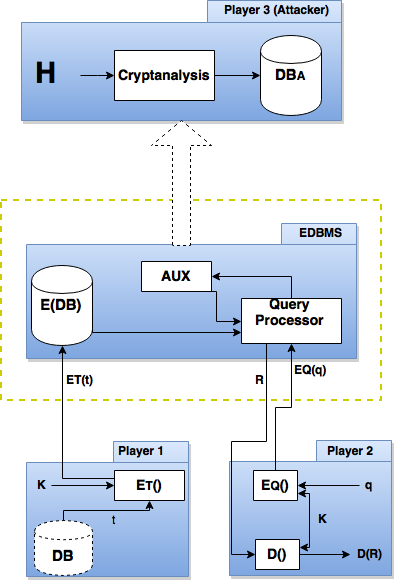
\includegraphics[scale=0.5]{SCONEDB}
     \caption{Figure 1: SCONEDB Model}
\end{figure}
Figure 1 shows SCONEDB model for encrypted database computation. Player 1 is the owner of a database $DB$ on which player 2 can execute certain queries. Instead of processing queries locally Player 1 exports $DB$ to $Encrypted Database Management System$(EDBMS) so Player 2 submits his queries to EDBMS to query DB of Player 1. To secure his data,Player 1 encrypts all tuples in $DB$ before sending them to EDBMS also Player 2 encrypts all his query . In this model EDBMS is considered \textit{trusted but curious}. EDBMS executes an encrypted query on the encrypted database and returns encrypted result $R$($R$ is a set of encrypted tuples which are the answer of a kNN query) to Player 2. To obtain plain result Player 2 applies a decryption function $D$ over $R$.
\\
In this SCONEDB model Player 1 and Player 2 have to agree on common $encryption scheme$. Also Player 1 and Player 2 can be the same actor. In SCONEDB an encryption scheme consists of the following components:
\begin{itemize}
\item \textit{Secret key K}. Encryption and decryption processes requires a key $K$. In this model key is kept private to Player 1 and Player 2.
\item \textit{Database encryption function $E_{T}()$}. The encrypted database $E(DB)$ is obtained by encrypting each tuple $t$ in $DB$ by $E_{T}(t,K)$.
\item \textit{Query encryption function $E_{Q}()$}. Each query $q$ is encrypted by $E_{Q}(q,K)$ before it is submitted to EDBMS
\item \textit{Result decryption function D()} .Each tuple $\hat{t}$ in the encrypted result $R$ is decrypted by $D(\hat{t},K)$
\item \textit{A set of auxiliary operators Aux}. An auxiliary operator
$A_e$ in $Aux$ operates on the encrypted database to obtain information for the purpose of answering queries. In our case $A_e$ returns Euclidean distance between an encrypted tuple $p$ and an encrypted query tuple $q$
\end{itemize}
The main goal in the SCONEDB model is to design an encryption scheme in which $Aux$ can operate on $E(DB)$ to support query processing.
\subsection{Attack models in encrypted databases}
When using SCONEDB model in designing our application we assume that the EDBMS is located at a third party . Therefore we assume that attacker (player 3) sees and controls the environment of EDBMS so attacker has accesses to the encrypted database ,encrypted queries and the ecnrypted results. Also we assume that attacker knows all the components of the scheme except the key. These include
the encryption and decryption procedures ($E_{T}(),E_{Q}()$ and $D()$) also the set of auxiliary operators $Aux$.Attacker's objectives is to recover a plain database $DB_A \subseteq DB$.We assume the attacker is capable to execute PTIME cryptanalysis algorithms with respect to the size of the encrypted database. Main objective is to deny the attacker from obtaining $DB_A$. To better evaluate the strength of an encryption scheme, we classify attackers into different levels based on the knowledge $H$ they possess.
\begin{itemize}
	\item Level 1:\textit{ the attacker observes only encrypted database $E(DB)$, i.e. $H=\langle E(DB) \rangle$. This corresponds to ciphertext-only attack (COA) in cryptography. In practice, there are applications accessed by secluded users, for which other can hardly observe any information other than encrypted data.}
	\item Level 2:\textit{ Apart from $E(DB)$, the attacker knows a set of plain tuples  $P$ in $DB$, but doesn't know their corresponding encrypted values in $E(DB)$, i.e. $H=\langle E(DB), P \rangle$. This corresponds to known-sample attacks in databases in literature. For example, if an attacker observes the encrypted database of a bank and some of his sources are his customers of the bank, he then knows the values of several tuples in the plain database.}
	\item Level 3:\textit{ Apart from $E(DB)$, the attacker knows a set of plain tuples  $P$ in $DB$ and he knows the corresponding encrypted values of those tuples, i.e. $H=\langle E(DB), P, I\rangle$, where $P \subset DB$ and $I(t)=E_T(t, K)$ for all $t \in P$. This corresponds to known known-plaintext attack in cryptography $(KPA)$ or known input-output attack in database literature. For example, if the attacker opens a new account in a bank, and observes only one new encrypted tuple afterwards, he can associate the new account's information (unencrypted) with the encrypted value of the new tuple.}
\end{itemize}
If an encryption scheme resists a higher level attack,it resists a lower level one as well.Level-2 attacks capture practical scenarios this is because in some applications, it is not difficult to observe a small number of plain database tuples. Note that level-3 attacks are rare in practice, since it is not
easy for someone who does not hold the encryption key to associate known plain tuples to their encrypted values.

\subsection{Distance Recoverable Encryption}
In kNN computation, distances between database points to a query point are computed for finding the nearer neighbors to the query point. To solve the secure kNN problem, it is natural to consider adopting an encryption scheme that allows
the system to compute $d(p_1,p_2)$ on $E(DB)$ for database points $p_1$ and $p_2$ in $DB$. Authors start with the definition of \textit{distance recoverability}.
\\
\\
DEFINITION 1 \textit{(Distance-recoverable encryption DRE)
Given an encryption function E and a key K, let E(p,K) be the encrypted value of a point p in DB. E is distance-recoverable if and only if there exists a computational procedure f such that $\forall p_{1},p_{2}, K, f(E(p_{1},K),E(p_{2},K))=d(p_{1},p_{2})$}.
\newline
\newline
Wong shows that DRE and hence DPT is not secure under level-2 or level3 attacks and introduces a theorem:
\\
\\
THEOREM 1 \textit{Assume a DRE E is used to encrypt DB to get E(DB). A level-3 attacker  with $\langle E(DB), P, I \rangle$ can recover DB if p contains  at least d+1 points $x_{i}$ ($1\le i \le d + 1$) such that the set of vectors $\{x_{j} - x_{i}	| 2 \le j \le d + 1\}$ are linearly independent.} 
\\
\\
\textit{PROOF}  Since the encryption is a DRE, the distance between any two points p and q, d(p, q), can be computed by the attacker using \textit{f(E(p, K), E(q, K))}.Suppose the attacker wants to find the original value of an encrypted point $y' \in E(DB)$. Let the set of known points in $P$ be $\{x_{1},x_{2},...,x_{d'+1}\}$ and $y$ be the original value of $y'$ before encryption . Attacker can set up $d+1$ equations : $d(x_{i},y) = f(I(x_i),y')$ for $i = \overline{1,d+1}$.Each equation thus represents a $d$-dimensional hypersphere. The solution of $y$ lies on the intersection of the hyperspheres.Since $y$ exists in the database, a solution must exist.Author show that if the set of vectors $\{x_j - x_1 \| 2\leq j\leq d_1\}$ are linearly independent, the $d+1$ hypersheres intersect at exactly one point so, $y$ can be uniquely determined. Hence the attacker can recover the entire database $ \square$
\\
\\
The level-3 attack shown above is independent of the implementation of DRE. So, no DRE (e.g. DPT) can survive this level-3 attack.
\subsection{Asymmetric Scalar-Product-Preserving Encryption}
The weakness of DRE comes from the fact that the attacker is able to recover
distance information from the encrypted database. More specifically, given any two points $p_1$ and $p_2$ in DB, their distance $d(p_1,p_2)$ can be determined from their encrypted values $E_T(p_1,K)$ and $E_T(p_2,K)$. In kNN search exact distance computation is not necessary we only need a distance comparation. Given two points $p_1$ and $p_2$ in $DB$ we must decide which of the two points is nearer to a query point q. Note that,
\begin{equation}
\begin{aligned}
d(p_1,q) &\geq d(p_1,q)\\
\sqrt{\left \| p_1 \right \|^2 - 2p_1\cdot q + \left \|q \right \|^2} &\geq \sqrt{\left \| p_2 \right \|^2 - 2p_2\cdot q + \left \|q \right \|^2} \\
\left \| p_1 \right \|^2 - \left \| p_2 \right \|^2 + 2(p_2 - p_1)\cdot q &\geq 0
\end{aligned}
\end{equation}
where $\left \| p \right \|$ represents the Euclidean norm of $p$ and $\cdot$ represents scalar product. $\left \| p \right \|^2$ cab be represented by $p\cdot p$. So, the inequality is decomposed to a number of scalar product computations. This suggests a scalar-product-preserving encryption $E_{spp}$ i.e. $\forall p_1, p_2 \in DB,p_1 \cdot p_2 = E_{spp}(p_1,K)\cdot E_{spp}(p_2,K)$,for kNN computation.
\\
\\
\\
THEOREM 2:\textit{Scalar-product-preserving encryption is distance recoverable.}
\\
\\
PROOF. Let $p'_1$ (resp $p'_2$) be the encrypted point of $p_1$(resp $p_2$) in $DB$. Define function $f$ by : \\
\begin{equation}
f(p'_1,p'_2)= \sqrt{p'_1\cdot p'_2 -2(p'_1\cdot p'_2) + p'_2\cdot p'_2}
\end{equation}
Since the encryption preserves scalar product ,we have RHS $=\sqrt{p_1\cdot p_2 -2(p_1\cdot p_2) + p_2\cdot p_2} = d(p_1,p_2)\square$
\\
Wong et al. define several scalar products:
\begin{itemize}
\item (type-1) scalar product of a database point with itself (e.g. $\left\|p\right\|^2$)
\item (type-2) scalar product of a database point with query point
\item (type-3) scalar product of two different database points $p_1$ and $p_2$
\end{itemize}
For our purpose we need an encryption that preserves type-2 but not type-1 or type-3 scalar products. With the precomputed type-1 scalar products, we can verify the inequality of Eq. 1 on the encrypted database to implement the distance comparison operation. Since the encryption does not preserve type-1 or type-3 products, it is not distance recoverable by design. The encryption is thus resilient to level-2 attacks.

DEFINITION 2: \textit{(Asymmetric scalar-product-preserving encryption (ASPE))}\\
\textit{Let E be an encryption function and E(p, K) be the encrypted value of a point p given a key K. E is an ASPE if and only if E preserves type-2 scalar products but not the other two types, i.e.}
\\
\textit{
\begin{enumerate}[(i)]
\item $p_i\cdot q = E(p_i,K)\cdot E(q,K)$ for any $p_i$ in DB and any query point q
\item $p_i\cdot p_j \neq E(p_i,K)\cdot E(p_j,K)$ for any $p_i$ and $p_j$ in DB.
\end{enumerate}}
In Definition 2, we require that the encrypted value of a query $q$ not equal to that of any point $p_j$ in $DB$,even when $q=p_j$.This suggests that query points and database points
should be encrypted differently.That is the encryption functions $E_T()$ and $E_Q()$ in the encryption scheme should be different.

The scalar product of $p$ and $q$ (represented by column vectors) can be represented as $p^{T}Iq$,where $p^T$ is the transpose of $p$ and $I$ is a $d \times d$ identity matrix. $I$ can be decomposed to $MM^{-1}$ for any invertible matrix $M$,i.e., $p^{T}q=(p^{T}M)(M^{-1}q)$. If we set $p' = E_T(p,K) = M^Tp$ (resp. $q' = E_q(q,K) = M^{-1}q$)  it is not possible for one to determine the value of $p$ (resp. $q$) from $p'$ (resp. $q'$) without knowing $M$. Also ,$p'^{T}q' = p^{T}MM^{-1}q = p^{T}q$ i.e , type-2 scalar product is preserved. Suppose $p'_1$ and $p'_2$ are the encrypted points of $p_1$ and $p_2$ in $DB$ respectively ,then $p'^{T}_{1}p'_{2} = p^{T}_{1}MM^{T}p_2$ which is not equal to $p_{1}^{T}p_2$ in general. Type-1 and type-3 scalar products therefore not preserved.So, we ASPE can be implemented by using $M$ and $M^{-1}$ as the transformations for database points and queries .



\subsection{A Secure Scheme Against Level-2 Attacks}
Wong idea is to treat a pre-computed type-1 scalar product $\left\|p\right\|^2$ as the $(d+1)$-st dimension of the point $p$. Given a( $d$-dimensional)  database point $p$ we create a $(d+1)$-dimensional point $\hat{p}$. The first $d$ dimensions of $\hat{p}$ are those of $p$, and the $(d+1)$-st dimension of $\hat{p}$ is set to $-0.5\left\|p\right\|^2$.The extended database points are then transformed(encrypted) using ASPE.

Similarly, we need to extend a query $q$ to a $d+1$-dimensional point $\hat{q}$ before applying ASPE. The simplest way is to set the $(d+1)$-st dimension of $\hat{q}$ to 1. The problem with this method is that the unencrypted query points $\hat{q}$'s all lie on a $d$-dimensional hyperplane with the unit vector in the $(d+1)$-st dimension being the normal of the hyperplane.The attacker can determine the normal of that hyperplane in the transformed space. By considering the normal in the original space and the normal in the transformed space, the attacker obtains some level-3-like information, which is undesirable.

To avoid this problem Wong introduces a random factor. For each query q is generated a random number $r >0$ and scale $\hat{q}$ by $r$, i.e.,$\hat{q} = r(q^T,1)^T$. In THEOREM 3 is shown that this scaling does not affect the correctness of the distance comparison operation
\begin{itemize}
\item \textbf{Key:} a $(d+1)\times (d+1)$ invertible matrix $M$.
\item \textbf{Tuple encryption function $E_T$ :} Consider a database point p
\begin{enumerate}
\item Create a $(d+1)-$dimensional point $\hat{p}$ = $(p^T,-0.5\left \| p \right \|^{2})^T$
\item The encrypted point $p' = M^T\hat{p}.$
\end{enumerate}
\item{\textbf{Query encryption function} $E_Q$}: Consider a query point q
\begin{enumerate}
\item Generate a random number $r > 0$
\item Create a $(d+1)$-dimensional point $\hat{q} = r(q^T,1)^T$
\item The encrypted query point $q' = M^{-1}\hat{q}$
\end{enumerate}
\item \textbf{Distance comparison operator} $A_e$: Let $p'_1$ and $p'_2$ be the encrypted points of $p_1$ and $p_2$ respectively. To determine whether $p_1$ is nearer to a query point $q$ than $p_2$ is, the system checks whether $(p'_1 - p'_2)\cdot q' > 0$,where $q'$ is the encrypted point of $q$.
\item \textbf{Decryption function} $D$: Consider an encrypted point $p'$. The original point $p=\pi_{d}M^{T^{-1}}p'$ where $\pi_d$ is a $d\times (d+1)$ matrix which projects on the first $d$ dimensions and $\pi_d = (I_d,0)$ where $I_d$ is the $d\times d$ identity matrix.
\end{itemize}
THEOREM 3. \textit{Suppose $p'_1$,$p'_2$ and $q'$ are the are the encrypted
points of the database points $p_1$,$p_2$ and the query point q, respectively, scheme correctly determines whether $p_1$ is closer to q than $p_2$ is by evaluating $(p'_1 - p'_2)\cdot q' > 0.$ }
\\
\\
\textit{PROOF:} Note that\\ 
\begin{center}
$(p'_1 - p'_2)\cdot q'$  =  $(p'_1 - p'_2)^T\cdot q'$  =  $(M^T \hat{p_1} -M^T \hat{p_2} )M^{-1}\hat{q}$  =  $(\hat{p_1}-\hat{p_2})^T\hat{q}$
\end{center}
The scalar product of these two $(d+1)$-dimensional points can be represented as:\\
\begin{center}
$(p_1 - p_2)^T(rq)+(-0.5 \left\| p_1\right\|^2 + 0.5\left\| p_2\right\|^2)r = 0.5r(\left\|p_2\right\|^2 -  \left\| p_1\right\|^2 +2(p_1-p_2)^{T}q) = 0.5r(d(p_2,q)-d(p_1,q))$
\end{center}
So, the condition is equivalent to:
\begin{center}
$0.5r(d(p_2,q)-d(p_1,q))>0 \Leftrightarrow (d(p_2,q)>d(p_1,q)\square$
\end{center}
\subsection{Random Asymmetric Splitting}
A level-3 attacker can compute matrix $M$ used in Scheme-1 by setting up enough number of equations using points in $P$ to solve for the unknowns in transformation. In order to make scheme harder to crack Wong et al proposed a method to introduce randomness into the scheme by splitting database point p at each dimension randomly.More specifically, we randomly generate two $d$-dimensional points $p_a$ and $p_b$ (called two $random$ $shares$)
such that for each dimension $i$, we have $p[i] = p_a[i] + p_b[i]$.For simplicity, we write $p = p_a + p_b$. Similarly query point $q$ is splitted. Query and database points can be splitted on each dimension using a split configuration. 
\begin{itemize}
	\item \textbf{Key} two $d' \times d'$ invertible matrices $M_1, M_2$; A bit string S of $d'$ bits: $S_i$ denotes  the $i$-th bit in $S$; $d'-(d+1)$ random numbers $w_{d+2}, w_{d+3},...,w_{d'}$. 
	\item \textbf{Tuple encryption function} $E_T$:	Let $p$ be a database point. 
	\begin{enumerate}
	\item Create a $d'$-dimensional point, where the first $d$ dimensions are copied from $p$. $\hat{p}[d+1]$ is set to $-0.5||p||^2$. For $i=d+2$ to $d'$, if $S_i=1$, we set $\hat{p}[i]$ to $w_i$; otherwise we set $\hat{p}[i]$ to a random number. For the last dimension with which $S_i=0, \hat{p}[i]$ is given a value so that the scalar product over the artificial attributes is 0, or formally $\frac{\sum_{i=d+1}^{s-1}w_it_i}{w_s}$. 
	\item Also we create two shares of $\hat{p}: \hat{p_a}$ and $\hat{p_b}$. For $i=1$ to $d'$, if $S_i=1$ we randomly split the value of $\hat{p}[i]$ into $\hat{p_a}[i]$ and $\hat{p_b}[i]$. If $S_i=0$, both $\hat{p_a}[i]$ and $\hat{p_b}[i]$ are set to $\hat{p}[i]$. 
	\item The encrypted value of $p$ is pair $(p'_a=M_1^T\hat{p}_a,p'_b=M_2^T\hat{p}_b)$. 
	\end{enumerate}
	\item \textbf{Query encryption function} $Q_T$: Let $q$ be a query point. 
	\begin{enumerate}
	\item We generate a random number $r>0$. Also we create a $(d')$-dimensional where the first $d$ dimensions are given by $rq$. The $d+1$-st dimension is set to $r$. For $i=d+2$ to $d'$, if $S_i=0$, we set $\hat{q}[i]$ to $w_i$; otherwise we set $\hat{q}[i]$ to a random number. For the last dimension with which $S_i=1, \hat{q}[i]$ is given a value so that the scalar product over the artificial attributes is 0, or formally $\frac{\sum_{i=d+1}^{s-1}w_it_i}{w_s}$.
	\item Also we create two shares of $\hat{q}: \hat{q_a}$ and $\hat{q_b}$. For $i=1$ to $d'$, if $S_i=0$ we randomly split the value of $\hat{q}[i]$ into $\hat{q_a}[i]$ and $\hat{q_b}[i]$. If $S_i=1$, both $\hat{q_a}[i]$ and $\hat{q_b}[i]$ are set to $\hat{q}[i]$.
	\item The encrypted value of $q$ is pair $(q'_a=M_1^{-1}\hat{q}_a,q'_b=M_2^{-1}\hat{q}_b)$.
	\end{enumerate}
	\item \textbf{Distance comparison function} $A_e$: Let $(p'_{1a},p'_{1b})$ and $(p'_{2a},p'_{2b})$ be encrypted values for database points $p_1$ and $p_2$ and $(q'_a, q'_b)$ encrypted value for query point $q$. The system will check whether $(p'_{1a} - p'_{2a}) \cdot q'_a + (p'_{1b} - p'_{2b}) > 0$. If this condition is true then $p_1$ is closer to $q$ than $p_2$. 
	\item \textbf{Decryption function} $D$: Let $(p'_a, p'_b)$ be an encrypted point. First, we recover two shares and extract the first d dimensions in it: $p_a=\pi_{d}M_1^{T^{-1}}p'_a$ and $p_b=\pi_{d}M_2^{T^{-1}}p'_b$ where $\pi_d$ is $d \times (d+1)$ dimensional matrix which projects on first $d$ dimensions. Then, $p[i]$ is equal to $p_a[i]$ if $S_i=0$; or $p_a[i]+p_b[i]$ if $S_i=1$.
\end{itemize}

Relative to this scheme next theorem is essential. 
\\
\\
THEOREM 6 \textit{Random Asymmetric Splitting is resilient against level 3 attacks if the attacker cannot derive the splitting configuration, i.e., the bit string S of the key in previous scheme.}
\\
\\
\textit{PROOF:} If we consider the knowledge of tha attacker to be $H=\langle E(DB), P, I\rangle$, without loss of generality, we assume $d'=d+1$, i.e., no artificial attributes are added. (The addition of artificial attributes will only increase the security of scheme). From definition of level 3 attacks, for any point $p_i \in P$, attacker knows encrypted values $(p'_{ia}, p'_{ib})$. If the attacker does not know the splitting configuration, he has to model $\hat{p_ia}$ and $\hat{p_ib}$ as two random $d'$-dimensional vectors. The equations for solving the transformation matrices are: $M_1^T\hat{p_a}=p'_a$ and $M_2^T\hat{p_b}=p'_b$, where $M_1$ and $M_2$ are two $d' \times d'$ unknown matrices. There are $2d'|P|$ unknowns in $\hat{p_{ia}}$ and $2d'^2$ unknowns in $M_1$ and $M_2$. Since there are only $2d'|P|$ equations, which are less than number of unknowns, the attacker does not have sufficient information to solve for the transformation matrices. Hence, second Wong scheme is resilient against this level-3 attack. $\square$ 

\section{Our contribution on fixing KPA attack on ASPE}
\subsection{Known-Plaintext Attack on Enhanced Asymmetric Scalar Product Preserving Encryption}
In this section we will review Chunsheng \cite{Chunsheng} proposed attack over Wong's second protocol. Despite the fact that his attack works over Wongs' protocol we will discuss some of his statements about it, that in our opinion are not true. But first we will start with his reasoning about security of mentioned by us, Wong's protocol.
The problem about security state of Wong's protocol starts with theorem 5 that we presented above. We will remember that the protocol supposed to be resilient if the attacker couldn't derive the splitting configuration string S. Chunsheng first observes that Wong builds his protocol on assumption that an attacker couldn't derive the splitting configuration. Immediately he propose an efficient algorithm that breaks splitting configuration by recovering first $d+1$ bits of $S$, by applying a set of linear equations. After that he propose a thesis that Wong's protocol can be broken even if the hypothesis from theorem 5 holds. Next we will discuss all these aspects.
\\
\\
THEOREM 6: \textit{Given $d'$ plaintext-ciphertext pairs $p^j, \bar{p}^j$ for EASPE, a polynomial time algorithm identifies the first $d+1$ bits of s.}
\\
\\
\textit{PROOF:} Through EASPE, we have $d'\ge d+1$. Without loss of generality, we consider $d'>d+1$. We discuss $d'=d+1$ next.
Given $p^j, \bar{p}^j$, $j \in d'$ with $\bar{p}^j=(\bar{p_a}^j=M^T\hat{p_a}^j,\bar{p_b}^j=M^T\hat{p_b}^j)$, we denote $p=(p^j)\in Q^{d \times d'}$ and $\bar{p_a}=(\bar{p_a}^j)$, $\bar{p_b}=(\bar{p_b}^j)$, $\hat{p_a}=(\hat{p_a}^j)$, $\hat{p_b}=(\hat{p_b}^j)$, $\hat{p}=(\hat{p}^j)\in Q^{d' \times d'}$, where $\hat{p}^j$ from $p^j$ in step 1 of encryption in Wong's protocol, and $\hat{p}_a^j, \hat{p}_b^j$ are generated from $\hat{p}^j$ in step 2 of encryption.
On the one hand, we have $\hat{p}[1..d,	.]=p$, and if $s[i]=0$, $i \in \langle d \rangle$, then $p[i,.]=\hat{p}[i,.]$; otherwise $\hat{p}[i,.]=\hat{p_a}[i,.] + \hat{p_b}[i,.]$, according to encryption step. That is, if $s[i]=0, i\in \langle d \rangle$, then $p[i,.]=\hat{p}_a[i,.]=\hat{p}_b[i,.]$; otherwise, $p[i,.]=\hat{p}_a[i,.]+\hat{p}_b[i,.]$. On the other hand, because $\bar{p}_a=M_1^T\hat{p}_a,\bar{p}_b=M_2^T\hat{p}_b$, when $\bar{p}_a,\bar{p}_b$ are invertible, we can solve equations $x \times \bar{p}_a=p[i,.], y \times \bar{p}_b=p[i,.]$, as well as determine $s[i]=0, i \in \langle d \rangle$ if $x \times \bar{p}_a^{new}=p^{new}[i]$ and $y \times \bar{p}_b^{new}=p^{new}[i]$, where $p^{new}, \bar{p}^{new}$ is a new plaintext-ciphertext pair. That is, identifying the value of s[i], $i \in d$ is easy. When $\{i|s[i]=0, i \in \langle d \rangle \setminus \langle d+1	\rangle\}$ is not an empty set; However, $\bar{p}_a, \bar{p}_b$ are not invertible by encryption. \newline
Next Chunsheng presents four arguments which proof we will not show here, that helps us to understand correctness of the attack. 
\begin{enumerate}
	\item \textit{Argument 1:} The rank of $\hat{p_a}, \hat{p_b}\bar{p_a}, \bar{p_b}$ are all $d'-1$ with probability 1.
	\item \textit{Argument 2:} An linear invertible linear transform $E$ exists, such that $E \times \hat{p_a}= \begin{pmatrix}
	\hat{p_a}[1..d'-1,.] \\ 0^{1 \times d'})
	\end{pmatrix}$ and $E \times \hat{p_b}= \begin{pmatrix}
		\hat{p_b}[1..d'-1,.] \\ 0^{1 \times d'})
	\end{pmatrix}$.
	\item \textit{Argument 3:} Let $K_1=M^T_1E^{-1}, K_2=M^T_2E^{-1}$. If $\bar{p_a}[1..d'-1], \bar{p_b}[1..d'-1]$, are invertible, then $K_1[1..d'-1],K_2[1..d'-1]$ are also invertible.
	\item \textit{Argument 4:} Assume $\bar{p_a}[1..d'-1],\bar{p_b}[1..d'-1]$ are invertible. Let $x=(\bar{x},0), y=(\bar{y},0)$, where $\bar{x}=(K_1[1..d'-1])^{-1}(i,.)=p[i,1..d'-1]\times (\bar{p_a}[1..d'-1])^{-1}, \bar{y}=(K_2[1..d'-1])^{-1}(i,.)=p[i,1..d'-1]\times (\bar{p_b}[1..d'-1])^{-1}$. If $x \times \bar{p_a}=p[i,.], y \times\bar{p_b}=p[i,.]$, then $s[i]=0, i \in \langle d \rangle$; otherwise $s[i]=1$. 
\end{enumerate}

Should be remarked to things: first is that if rank of $\hat{p_a}, \hat{p_b}\bar{p_a}, \bar{p_b}$ are less than $d'-1$, then we should choose again plaintext-ciphertext pairs, until condition is satisfied. Also we should be aware that if $d'=d+1$, then there are not $w_i$ random values in ciphertexts, and determining the bit values of $s$ is also easy. We assume that $\bar{p_a}=M^T_1 \times \hat{p_a}, \bar{p_b}=M^T_2 \times \hat{p_b}$ are inverse because we can choose arbitrary plaintext-ciphertext pairs. Then, we obtain another test set $\{q, (\bar{q_a},\bar{q_b})\}$ of plaintext-ciphertext pairs and compute $q'=p \times \bar{p_a}^{-1} \times \bar{q_a}$. if the $i$th row of $q'$ is equal to to $i$th row of $q$, then $s[1]=0$ else $s[1]=1$. \newline
Using this technique, we can find only the first $d+1$ bits of $s$, that means that we cannot decrypt encrypted data from database. But Chunsheng presents another attack that uses information found in attack above in order to find a secret key.
\\

THEOREM 7: \textit{Given $2d'$ plaintext ciphertext pairs $p^j, \bar{p}^j$, a polynomial time algorithm solves a secret key in EASPE.}
\\

\textit{PROOF:} Consider $\bar{p}^j=(\bar{p_a}^j=M^T_1\hat{p_a}^j,\bar{p_b}^j=M^T_2\hat{p_b}^j), j \in \langle2d' \rangle, \bar{p_a}=(\bar{p_a}^1,\bar{p_a}^2,...,\bar{p_a}^{2d'}), \bar{p_b}=(\bar{p_b}^1,\bar{p_b}^2,...,\bar{p_b}^{2d'}), \hat{p_a}=(\hat{p_a}^1,\hat{p_a}^2,...,\hat{p_a}^{2d'}),\hat{p_b}=(\hat{p_b}^1,\hat{p_b}^2,...,\hat{p_b}^{2d'}), \hat{p}=(\hat{p}^1,\hat{p}^2,...,\hat{p}^{2d'}), p=(p^1,p^2,...,p^{2d'})$.

In order to identify the secret key, we first will use the first $d$ bites using technique from proof from theorem 6. Having the first $d$ bits of $s$, we can solve the secret key for different bit values of $s[i], i \in \langle d \rangle$ 
\begin{enumerate}
	\item Secret key for $s[i]=0, i \in \langle d \rangle$: for $s[i]=0, i \in \langle d \rangle$ the secret key is determined by solving equations $x=(\bar{x},0), y=(\bar{y},0)$, where $\bar{x}$ and $\bar{y}$ are determined by using argument 4.
	\item Secret key for $s[i]=0, i \in \langle d \rangle$: using encryption from Wong's scheme we have $\bar{p}_a=M^T_1\hat{p}_a,\bar{p}_b=M^T_2\hat{p}_b$ and $\hat{p}_a[i,.] + \hat{p}_b[i,.]=\hat{p}[i,.]=p[i]$ for $s[i]=1, i \in \langle d\rangle$, Thus for $s[i]=1, i \in \langle d\rangle$, we have: $(M_1^T)^{-1}[i,.]\times\bar{p}_a + (M_2^T)^{-1}[i,.]\times\bar{p}_b = p[i,.] \Leftrightarrow 
	\begin{pmatrix}
	(M_1^T)^{-1}[i,.],(M_2^T)^{-1}[i,.] 
	\end{pmatrix} \times \begin{pmatrix}
	\bar{p}_a\\
	\bar{p}_b
	\end{pmatrix}=p[i,.]$ \\
	If $\hat{p}_{ab} = \begin{pmatrix}
	\hat{p}_a\\
	\hat{p}_b
	\end{pmatrix}$ is an invertible matrix, then we can directly solve $\begin{pmatrix}
		(M_1^T)^{-1}[i,.],(M_2^T)^{-1}[i,.] 
	\end{pmatrix}$, but $\hat{p}_{ab}$ is not invertible.
\end{enumerate}

Chunsheng presents four arguments that help us solve problem above. We will skip their proofs.
\begin{enumerate}
	\item \textit{Argument 5:} Let $\epsilon_0=|\{i|s[i]=0, i \in \langle d'\rangle\}|, \epsilon_1=|\{i|s[i]=1, i \in \langle d'\rangle \setminus \langle d + 1\rangle \}|$. The ranks of $\bar{p}_{ab}, \hat{p}_{ab}$ are all $2d' - \epsilon_0 -\epsilon_1$ with probability 1.
	\item \textit{Argument 6:} An invertible linear transform $E$ exists, such that \\
	$\bar{p}_ab=\begin{pmatrix}
	M^T_1E^{-1}&&&		0\\
	0	&&&	M^T_2E^{-1} 
	\end{pmatrix} \times \begin{pmatrix}
	E 	&&&	0\\
	0	&&&	E
	\end{pmatrix}\hat{p}_{ab} = 
	\begin{pmatrix}
	K_1 	&&&	0\\
	0	&&&	K_2
	\end{pmatrix}
	\begin{pmatrix}
	\hat{p}_a[1..(d'-1)] 	\\
	0^{1 \times2d'}	\\
	\hat{p}_b[1..(d'-1)]	\\
	0^{1 \times2d'}	\\
	\end{pmatrix}$ .
	\item \textit{Argument 7:} Let $\bar{\bar{p}}_{ab}=
	\begin{pmatrix}
	\bar{p}_a[1..(d'-1),1..(2d'-2)] 	\\
	\bar{p}_b[1..(d'-1),1..(2d'-2)]	\\
	\end{pmatrix},
	\hat{\hat{p}}_{ab}=
	\begin{pmatrix}
	\hat{p}_a[1..(d'-1),1..(2d'-2)] 	\\
	\hat{p}_b[1..(d'-1),1..(2d'-2)]	\\
	\end{pmatrix},
	\bar{K} =
	\begin{pmatrix}
	K_1 	&&&	0\\
	0	&&&	K_2
	\end{pmatrix},
	\bar{\bar{K}}=
	\begin{pmatrix}
	K_1[1..(d'-1)] 	&&&
	0	\\
	0&&&
	K_2[1..(d'-1)]
	
	\end{pmatrix} .
	$ An invertible linear transform exists, such that \\
	$\bar{\bar{P}}_{ab}=\bar{\bar{K}}F^{-1} \times F \hat{\hat{P}}_{ab}=\bar{\bar{K}}F^{-1}\times
	\begin{pmatrix}
	\hat{p}[1..d,1..(2d'-2)] 	\\
	\hat{p}_a[d+1..d'-1,1..(2d'-2)]	\\
	\hat{p}_b[1..d'-\epsilon_1 -\epsilon_0 + 1,1..(2d'-2)]	\\
	0^{(\epsilon_1+\epsilon_0-2)\times(2d'-2)} 
	\end{pmatrix} = 
	\bar{\bar{K}}F^{-1}\times
	\begin{pmatrix}
		p[1..d,1..(2d'-2)] 	\\
		\hat{p}_a[d+1..d'-1,1..(2d'-2)]	\\
		\hat{p}_b[1..d'-\epsilon_1 -\epsilon_0 + 1,1..(2d'-2)]	\\
		0^{(\epsilon_1+\epsilon_0-2)\times(2d'-2)} 
	\end{pmatrix}$.
	\item \textit{Argument 8:} Consider $K=\bar{\bar{K}}F^{-1}$ and $\sigma=2d'-\epsilon_1-\epsilon_0$. We assume that $\bar{\bar{p}}_{ab}[1..\sigma]$ is invertible. For $s[i]=1, i\in \langle d\rangle$, the secret key is $(x \hspace{0.2cm} y) = (\bar{\bar{x}}[1..(d'-1)] \hspace{0.2cm} 0^{1 \times 1} \hspace{0.2cm} \bar{\bar{x}}[d'..\sigma]$ $\hspace{0.2cm} 0^{1 \times(\epsilon_0 + \epsilon_1 - 1)})$, such that $(x \hspace{0.2cm} y) \times \bar{p}_{ab}=p[i,.]$, where $\bar{\bar{x}}=(K[1..\sigma])^{-1}[1,.]=p[i,1..\sigma]\times (\bar{\bar{p}}_{ab}[1..\sigma])^{-1}$. 
\end{enumerate}

\subsection{Fixed protocol}
In this section we present our fix for Chunsheng attack on ASPE.

\begin{itemize}
	\item{\textbf{Key}}
	Given parameters $\lambda$,$\beta$ the dimensions $d(\lambda)$,$d'(\lambda)$ of a database point $p$, and encrypted value of $p$:
	
	\begin{enumerate}
		\item Choose two invertible matrices $M_{1},M_{2}\in Q^{d' \times d'}$ , such that $\left |M_{k}\left [ i,j \right ]  \right | \leq 2^{\lambda} , k \in \left \langle2 \right \rangle i,j \in \left \langle d' \right \rangle $
		
		\item Randomly generate bit string $s$,$\in \left \{ 0,1\right \}^{d'-(d+1)}$ 
		\item Choose $d' - \left ( d+1 \right )$ random numbers $w_{d+2},w_{d+3}, \ldots ,w_{d'} \in Q$ such that $w_{j} \ne 0$ and $\left | w_{j} \right | \leq 2^{\lambda},j \in \left \langle d' \right \rangle \setminus  \left \langle d+1 \right \rangle$
		
		\item Choose a permutation matrix $P_{\pi},P_{\pi} \in \left\{0,1\right\}^{d' \times d'}$ 
		such that $\nexists P_{\pi}\left[i,i\right] = 1, \nexists P_{\pi}\left[i,j\right] =P_{\pi}\left[i,k\right] = 1, j\neq k$ and $\nexists P_{\pi}\left[i,j\right] =P_{\pi}\left[k,j\right] = 1, i\neq k ;i,j,k\in \left \langle d'\right \rangle$
		\item Output secret key $sk = \left \{ M_{1} ,M_{2} ,s ,\left \{ w_{j},j \in \left \langle d' \right \rangle \setminus \left \langle d+1 \right \rangle \right \},P_{\pi} \right  \}$
	\end{enumerate}
	
	\item{\textbf{Encryption algorithm}}
	Given a $d$-dimensional database point $p$ and secret key $sk$:
	\begin{enumerate}
		\item Create a $d'$-dimensional $\tilde p$:
		\begin{itemize}
			\item $\tilde{p}[i] = p[i],\forall i \in \left \langle d \right \rangle$
			\item $\tilde{p}[d+1] = -0.5\left \|  p\right \|^{2}$
			\item
			$\left\{\begin{matrix}
			\tilde{p}[i] = w_i,if\;s[i] = 1 & &\\ 
			& & ,i\in \left \langle d' \right \rangle \setminus  \left \langle d+1 \right \rangle \\
			\tilde{p}[i] = r_i,if\;s[i] = 0 & &
			\end{matrix}\right.$
			\\
			\\
			where $r_i\in Q$ and $\left|r_i\right|\leq 2^\lambda$;
			\item
			Let k = $max\left \{ j\mid s\left [ j \right ] = 0,j\in\left \langle d' \right \rangle\setminus \left \langle d+1 \right \rangle \right \}$
			\\
			\\
			$    \tilde{p}\left [ k \right ] = -\left ( \sum\limits_{s_j=0,j\geq d+2,j\neq k}^{}\tilde{p}\left [ j \right ]w_j\right)/w_k$
		\end{itemize}
		\item
		Permute $\tilde{p}$ using $P_\pi$:
		\begin{itemize}
			\item 
			$\hat{p} =\tilde{p}^{T}P_\pi $
		\end{itemize}
		\item
		Split $\hat{p}$ into $\hat{p}_a$ and $\hat{p}_b$ using $s$:
		\begin{itemize}
			\item Randomly choose $R \in Q^{n}$,such that $0<\left | R\left [ i \right ]  \right | \leq 2^\lambda ,i \in \left \langle d' \right \rangle$ 
			
			\item 
			$\left\{\begin{matrix}
			\hat{p_a}\left [ i \right ] = \hat{p}\left [ i \right ] + R\left [ i \right ],& \hat{p_b}\left [ i \right ] = \hat{p}\left [ i \right ] - R\left [ i \right ],&if\,\,s\left [ i \right ]=1 &\\ 
			& & &,i\in \left \langle d' \right \rangle  \\
			\hat{p_a}\left [ i \right ] = \hat{p}\left [ i \right ] - R\left [ i \right ],&
			\hat{p_b}\left [ i \right ] = \hat{p}\left [ i \right ] + R\left [ i \right ],&if\,\,s\left [ i \right ]=0 &
			\end{matrix}\right.$
		\end{itemize}
		\item
		Generate encrypted value of $p$:
		\begin{itemize}
			\item $\overline{p}=\left ( \overline{p}_{a} = M^{T}_{1}\hat{p}_{a},\overline{p}_{b} = M^{T}_{2}\hat{p}_{b}\right )$
		\end{itemize}
	\end{enumerate}
	
	\item{\textbf{Query encryption algorithm}}
	Given a $d$-dimensional query point $q$ and secret key $sk$:
	\begin{enumerate}
		\item Create a $d'$-dimensional $\tilde q$:
		\begin{itemize}
			\item Choose randomly $r\in Q$ with $0<r\leq 2^\lambda$
			\item $\tilde{q}[i] = rq[i],\forall i \in \left \langle d \right \rangle$
			\item $\tilde{q}[d+1] = r$
			\item
			$\left\{\begin{matrix}
			\tilde{p}[i] = w_i,if\;s[i] = 0 & &\\ 
			& & ,i\in \left \langle d' \right \rangle \setminus  \left \langle d+1 \right \rangle \\
			\tilde{p}[i] = r_i,if\;s[i] = 1 & &
			\end{matrix}\right.$
			\\
			\\
			where $r_i\in Q$ and $\left|r_i\right|\leq 2^\lambda$;
			\item
			Let k = $max\left \{ j\mid s\left [ j \right ] = 1,j\in\left \langle d' \right \rangle\setminus \left \langle d+1 \right \rangle \right \}$
			\\
			\\
			$    \tilde{q}\left [ k \right ] = -\left ( \sum\limits_{s_j=0,j\geq d+2,j\neq k}^{}r_{j}w_j\right)/w_k$
		\end{itemize}
		\item
		Permute $\tilde{q}$ using $P_\pi$:
		\begin{itemize}
			\item 
			$\hat{q} =\tilde{q}^{T}P_\pi $
		\end{itemize}
		\item
		Split $\hat{q}$ into $\hat{q}_a$ and $\hat{q}_b$ using $sw$:
		\begin{itemize}
			\item 
			
			$\hat{q_a}\left [ i \right ] = \hat{q}\left [ i \right ],\hat{q_b}\left [ i \right ] = \hat{q}\left [ i \right ] ,i\in \left \langle d' \right \rangle  \\
			.$
		\end{itemize}
		\item
		Generate encrypted value of $q$:
		\begin{itemize}
			\item $\overline{q}=\left ( \overline{q}_{a} = M^{-1}_{1}\hat{q}_{a},\overline{q}_{b} = M^{-1}_{2}\hat{q}_{b}\right )$
		\end{itemize}
	\end{enumerate}
	\item{\textbf{Decryption algorithm }}: $D$ Let $(p'_a, p'_b)$ be an encrypted point. First, we recover two shares and extract the first d dimensions in it: $p_a=\pi_{d}M_{1}^{T^{-1}}(p'_a\cdot P_{\pi}^T)$ and $p_b=\pi_{d}M_{2}^{T^{-1}}(p'_b\cdot P_{\pi}^T)$ where $\pi_d$ is $d \times (d+1)$ dimensional matrix which projects on first $d$ dimensions. Then, $2p[i]$ is equal to $(p_a[i]+p_b[i])$. 
	\item{\textbf{Distance comparison algorithm}}
	Given the encrypted value $\overline{p}^{j} = \left ( \overline{p}^{j}_{a}, \overline{p}^{j}_{b}\right ),\overline{q}^{j} = \left ( \overline{q}_{a}, \overline{q}_{b}\right )$ of two database points $p_j,j\in \left \langle 2 \right \rangle$,a query point $q$:
	\begin{itemize}
		\item if $\left ( \overline{p}_{a}^{1} - \overline{p}_{a}^{2} \right )\overline{q}_{a}
		+ \left ( \overline{p}_{b}^{1} - \overline{p}_{b}^{2} \right )\overline{q}_{b} > 0$ then $p_1$ is nearer to $q$;otherwise $p_2$ is nearer to $q$.
	\end{itemize}
\end{itemize}
\subsection{Correctness proof}
Now we will discuss correctness of our algorithm. There are several aspects that we should present related to second Wong protocol. First of all we should make more clear what exactly make it vulnerable. The answer at this question is exposed in theorem 6. \\

So, what is the problem with Wongs' protocol. Answer is simple, it allows an attacker to make distinction between cases when bit values of split configuration string $s$ are used. So in our opinion, the phase that implies split of extended point can be done somehow different. This we showed in our fix. Also this fix implies change of query encryption algorithm. Now we will present our proof for search correctness using scheme above. After we made this proof, we observed that there can be done several changes in order to improve security. We will discuss these improvements later.
\\
\\
\textit{PROOF:} Let $(p'^1_a, p'^1_b)$ be the encrypted value for database point $p^1$, $(p'^2_a, p'^2_b)$ be the encrypted value for database point $p^2$ and $(q'_a, q'_b)$ be the encrypted value for a query point $q$.
\begin{center}
	$(p'^1_a-p'^2_a)q'_a+(p'^1_b-p'^2_b)q'_b>0$ 
	\newline
	\newline
	$(M^T_1\hat{p}_a^1-M^T_1\hat{p}_a^2)^TM^{-1}_1\hat{q}_a + (M^T_2\hat{p}_b^1-M^T_2\hat{p}_b^2)^TM^{-1}_2\hat{q}_b >0$
	\newline
	\newline
	$(\hat{p}_a^1-\hat{p}_a^2)^T\hat{q}_a +(\hat{p}_b^1-\hat{p}_b^2)^T\hat{q}_b >0$
	\newline
	\newline
	
\end{center}
Now, given splitting configuration string, given value on index $i, s[i], i \in \langle d\rangle$, our equation has following behavior:
	\begin{enumerate}
		\item if $s[i]=0$:
		\begin{center}
					
		  $(\hat{p}^1[i] + r^1[i]-\hat{p}^2[i] - r^2[i])^T(\hat{q}[i] - r^3[i]) +
		  (\hat{p}^1[i] - r^1[i] + \hat{p}^2[i] + r^2[i])^T(\hat{q}[i] + r^3[i]) >0$\newline
		  \newline
		  $\hat{p}^1[i](\hat{q}[i] - r^3[i]) + 
		  r^1[i](\hat{q}[i] - r^3[i]) -
		  \hat{p}^2[i](\hat{q}[i] - r^3[i]) - 
		  r^2[i](\hat{q}[i] - r^3[i]) +
		  \hat{p}^1[i](\hat{q}[i] + r^3[i]) - 
		  r^1[i](\hat{q}[i] + r^3[i]) - 
		  \hat{p}^2[i](\hat{q}[i] + r^3[i]) + 
		  r^2[i](\hat{q}[i] + r^3[i]) >0$
		  \newline
		  \newline
		  $\hat{p}^1[i]\hat{q}[i] - \hat{p}^1[i]r^3[i] + 
		  r^1[i]\hat{q}[i] - r^1[i]r^3[i] -
		  \hat{p}^2[i]\hat{q}[i] + \hat{p}^2[i]r^3[i] - 
		  r^2[i]\hat{q}[i] + r^2[i]r^3[i] +
		  \hat{p}^1[i]\hat{q}[i] + \hat{p}^1[i]r^3[i]) - 
		  r^1[i]\hat{q}[i] - r^1[i]r^3[i] - 
		  \hat{p}^2[i]\hat{q}[i] - \hat{p}^2[i]r^3[i] + 
		  r^2[i]\hat{q}[i] + r^2[i]r^3[i] >0$
		  \newline
		  \newline
		  $\hat{p}^1[i]\hat{q}[i]  
		  - r^1[i]r^3[i] -
		  \hat{p}^2[i]\hat{q}[i]  
		  + r^2[i]r^3[i] +
		  \hat{p}^1[i]\hat{q}[i]  
		  - r^1[i]r^3[i] + 
		  \hat{p}^2[i]\hat{q}[i] + 
		  r^2[i]r^3[i] >0$
		  \newline
		  \newline
		  $2\hat{p}^1[i]\hat{q}[i]  
		  - 2r^1[i]r^3[i] -
		  2\hat{p}^2[i]\hat{q}[i]  
		  + 2r^2[i]r^3[i]>0$ 
		  \newline
		  \newline
		  $\hat{p}^1[i]\hat{q}[i]  
		  - r^1[i]r^3[i] -
		  \hat{p}^2[i]\hat{q}[i]  
		  + r^2[i]r^3[i]>0$ 
		  \newline
		  \newline
  		  $\hat{p}^1[i]\hat{q}[i]  -
  		  \hat{p}^2[i]\hat{q}[i]  >r^1[i]r^3[i] - r^2[i]r^3[i]$
		  \newline
		  \newline
		  $(\hat{p}^1[i]-\hat{p}^2[i])\hat{q}[i]>r^1[i]r^3[i] - r^2[i]r^3[i]$
		  \newline
		  \newline
		\end{center}
		\item if $s[i]=1$:
		\begin{center}
			
			$(\hat{p}^1[i] - r^1[i]-\hat{p}^2[i] + r^2[i])^T(\hat{q}[i] + r^3[i]) +
			(\hat{p}^1[i] + r^1[i] - \hat{p}^2[i] - r^2[i])^T(\hat{q}[i] - r^3[i]) >0$\newline
			\newline
			$\hat{p}^1[i](\hat{q}[i] + r^3[i]) - 
			r^1[i](\hat{q}[i] + r^3[i]) -
			\hat{p}^2[i](\hat{q}[i] + r^3[i]) + 
			r^2[i](\hat{q}[i] + r^3[i]) +
			\hat{p}^1[i](\hat{q}[i] - r^3[i]) + 
			r^1[i](\hat{q}[i] - r^3[i]) - 
			\hat{p}^2[i](\hat{q}[i] - r^3[i]) - 
			r^2[i](\hat{q}[i] - r^3[i]) >0$
			\newline
			\newline
			$\hat{p}^1[i]\hat{q}[i] + \hat{p}^1[i]r^3[i] - 
			r^1[i]\hat{q}[i] - r^1[i]r^3[i] -
			\hat{p}^2[i]\hat{q}[i] - \hat{p}^2[i]r^3[i] + 
			r^2[i]\hat{q}[i] + r^2[i]r^3[i] +
			\hat{p}^1[i]\hat{q}[i] - \hat{p}^1[i]r^3[i]) + 
			r^1[i]\hat{q}[i] - r^1[i]r^3[i] - 
			\hat{p}^2[i]\hat{q}[i] + \hat{p}^2[i]r^3[i] -
			r^2[i]\hat{q}[i] + r^2[i]r^3[i] >0$
			\newline
			\newline
			$\hat{p}^1[i]\hat{q}[i]  
			- r^1[i]r^3[i] -
			\hat{p}^2[i]\hat{q}[i]  
			+ r^2[i]r^3[i] +
			\hat{p}^1[i]\hat{q}[i]  
			- r^1[i]r^3[i] + 
			\hat{p}^2[i]\hat{q}[i] + 
			r^2[i]r^3[i] >0$
			\newline
			\newline
			$2\hat{p}^1[i]\hat{q}[i]  
			- 2r^1[i]r^3[i] -
			2\hat{p}^2[i]\hat{q}[i]  
			+ 2r^2[i]r^3[i]>0$ 
			\newline
			\newline
			$\hat{p}^1[i]\hat{q}[i]  
			- r^1[i]r^3[i] -
			\hat{p}^2[i]\hat{q}[i]  
			+ r^2[i]r^3[i]>0$ 
			\newline
			\newline
			$\hat{p}^1[i]\hat{q}[i]  -
			\hat{p}^2[i]\hat{q}[i]  >r^1[i]r^3[i] - r^2[i]r^3[i]$
			\newline
			\newline
			$(\hat{p}^1[i]-\hat{p}^2[i])\hat{q}[i]>r^1[i]r^3[i] - r^2[i]r^3[i]$
			\newline
			\newline
		\end{center}		
	\end{enumerate}
From proof above we observe several things. First one is that it doesn't matter if $s[i]=1$ or $s[i]=0$, we obtain same result $(\hat{p}^1[i]-\hat{p}^2[i])\hat{q}[i]>r^1[i]r^3[i] - r^2[i]r^3[i]$, where $r^1[i]$ is random used at splitting step in datapoint encryption phase for point $p_1$, $r^2[i]$ is random used at splitting step in datapoint encryption phase for point $p_2$ and $r^3[i]$ is random used at splitting step in query encryption phase for point $q$. That is, in order to make right hand part of final expression 0, we should make $r^1[i]$ and $r^2[i]$ equal or $r^3[i]$ 0. In more concise terms that mean that we could not randomize query $q$ at split phase in encryption step. If we do so, this gives us freedom to not use a vector of random values in key. In our opinion this is a wise move, because it gives us possibility to randomize database points at encryption step. On the other hand we can have the mentioned above vector of random values inserted in key, and use it only in encryption phase where each extended will be built with the same random values.\\

If we will not respect this simple steps, asymmetric scalar product encryption will work, but will not have proper distance comparison properties, which is essential in our scenario. However, we showed that our changes to Wong's protocol are not changing its behavior and represent a fix for Chunsheng attack because changes that are made at splitting step in encryption phase are similar from the attacker point of view. This mean that he shouldn't be able to recover splitting configuration string and should not be able to use it in his way of recovering secret key, and of course to recover plain database data.

\section{Practical implementation}
In this section I present how we can use ASPE in securing databases and queries over them. To implement ASPEDB I use .Net framework and C\# as programming language.
I choose .NET because this framework have this advantages over other frameworks:
\begin{itemize}
\item \textbf{Interoperability:}.NET Framework provides means to access functionality implemented in newer and older programs that execute outside .NET environment. 
\item \textbf{Language independence:}.NET Framework supports the exchange of types and object instances between libraries and applications written using any conforming .NET language.
\item \textbf{Portability:} Microsoft submitted the specifications for CLI,C\# and C++/CLI to both ECMA\footnote{European Computer Manufacturers Association- international private (membership-based) non-profit standards organization} and ISO\footnote{International Organization for Standardization - international standard-setting body composed of representatives from various national standards organizations.} this makes it possible for third parties to create compatible implementations of the framework and its languages on other platforms.
\item \textbf{Security:} .NET offers a set of tools to prevent execution of code by the entities without permission.
\item \textbf{Simplified deployment:}.NET Framework includes design features and tools which help manage the installation of computer software to ensure that it does not interfere with previously installed software, and that it conforms to security requirements.
\end{itemize}
To store data I use MongoDB\footnote{https://www.mongodb.org official website} noSql database. MongoDB is a document database that provides high performance, high availability, and easy scalability. MongoDB advantages:
\begin{itemize}
\item Document Database
\begin{itemize}
\item Documents (objects) map nicely to programming language data types.
\item Embedded documents and arrays reduce need for joins.
\item Dynamic schema makes polymorphism easier.
\end{itemize}
\item High Performance
\begin{itemize}
\item Embedding makes reads and writes fast.
\item Indexes can include keys from embedded documents and arrays.
\item Optional streaming writes (no acknowledgments).
\end{itemize}
\item High Availability
\begin{itemize}
\item Replicated servers with automatic master failover.
\end{itemize}
\item Easy Scalability
\begin{itemize}
\item Automatic sharding distributes collection data across machines.
\item Eventually-consistent reads can be distributed over replicated servers.
\end{itemize}
\item Advanced Operations
\begin{itemize}
\item With MongoDB Management Service (MMS) MongoDB supports a complete backup solution and full deployment monitoring.
\end{itemize} 
\end{itemize}
\pagebreak{}
\subsection{ASPE DataBase}
In this section we will discus in detail ASPEDB implementation. ASPEDB is divided in three modules: application offers friendly graphical user interface that allows user to interact with database,web server that processes user requests and operates with database,database stores user data. Application is implemented using WPF\footnote{Windows Presentation Foundation} because it offers possibility to create attractive and intuitive GUI\footnote{Graphical User Interface}.Web Server hosts a WCF\footnote{Windows Communication Foundation} that is used to implement and deploy a service-oriented architecture (SOA). WCF exposes a set of methods for user to operate with encrypted DB. WCF is designed using service-oriented architecture principles to support distributed computing where services have remote consumers. Clients can consume multiple services; services can be consumed by multiple clients.This feature allow us to operate on multiple databases 

\begin{figure}[h!]
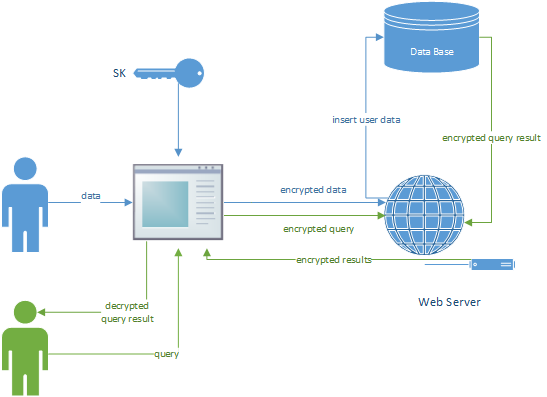
\includegraphics{application}
 \caption{ASPEDB application diagram}
\end{figure}

\pagebreak{}
\subsection{Data type conversion}
In ASPE data points are represented as vectors in $\mathbb{Q}^n$ but we need to store programming language data types such as numeric(byte,char,int,decimal), string and others (date,boolean) so we need to convert data types in numeric vectors with the possibility of converting data back. First we need to convert user data into a number(for numeric types its obvious) for strings(we allow only lowercase letters) we will encode each character in 2 decimal number and then concatenate them into a number $value = en(str[1]) \| en(str[2])\| \dots \|en(str[n])$ where $en$ is a function that encodes a character in a number for example we can set $en(ch) = ASCII(ch) -  87$. 

\begin{tabular}{ l | l || l | l}
 \hline		
 Char & Encoding & Char & Encoding \\ \hline
a	&	10	& 	n	&	23	\\
b	&	11	&	o	&	24	\\
c	&	12	&	p	&	25	\\
d	&	13	&	q	&	26	\\
e	&	14	&	r	&	27	\\
f	&	15	&	s	&	28	\\
g	&	16	&	t	&	29	\\
h	&	17	&	u	&	30	\\
i	&	18	&	v	&	31	\\
j	&	19	&	w	&	32	\\
k	&	20	&	x	&	33	\\
l	&	21	&	y	&	34	\\
m	&	22	&	z	&	35	\\
 \hline  
\end{tabular}
\newline


For example string $"abc"$ will be converted in number $101112$. To allow string alphabetical comparison we will set a maximum string length and pad our converted string with $0$ to the right so each value has the same number of digits. Boolean values($true,false$) could be converted as $true=1,false=0$. Date values will be converted as UNIX-time \footnote{\url{https://en.wikipedia.org/wiki/Unix_time}}. After values are converted as number we need to generate a point that will be encrypted using ASPE, for that we will create a point $p$ of dimension $d$ $\left [\underset{d}{\underbrace{ 0,0,\dots,value }}\right ]$. We observe that point $p$ is padded with $0$ to the left to improve security we can use a random vector $P\in \mathbb{Q}^n$ ,that will be part of secret key,instead of padding with 0 . Also this approach will be used in query transformation. 

By converting all of the data types to number we now can process queries and support comparing operations such as $<,\leq,=,>,\ge,\neq$ also I will show how to build more complex queries that allow us to search points that are in interval given by the user.
\pagebreak{}
\subsection{Points and Queries in ASPEDB}
Query coverage 
Each record inserted in data base by the users is a tuple $(Type,Name,Value)$ where $Type$ is data type of that record ,$Name$ is the name of record("column") and $Value$ is value of record. Records in db are encrypted using ASPE so each element in tuple is a point .The query that is used to obtain data from database is a tuple
\\$(Type,Name,Operator,Value,OptionalValue)$ where $Type$ is type of required point ,$Name$ is the name of required record ,$Operator$ is an comparison operator ,this operator is not encrypted so web service can determine when a query covers a record in database, $Value$ and $OptionalValue$ are used in comparison.Each element in tuple is a query point.
A query $q = (Type_q,Name_q,Operator,Value_q,OptionalValue_q)$ covers a record $r=(Type_r,Name_r,Value_r)$  if $Type_q = Type_r$ and $Name_q = Name_r$ and $Operator(Value_q,Value_r)$ and\\ $Operator(OptionalValue_q,Value_r)$.


In section 3 we presented a function \textit{Distance  comparison  algorithm} which determines which point is nearer to query. In data base we need to determine if a single point is covered by query , so we need to change the method generating point from user data. After we convert user data to a number and generate a point $p$ user selects a random number $s$($s>0$) and computes $c=p-s$ and $d=p+s$ so user hides value of $p$ in the middle of the interval $[c,d]$. After that user can encrypt points $c$ and $d$ using ASPE.
When web service need to check if a query $q$ covers a record($c,d$) he simply calculates:

\begin{itemize}
\item Equality filtering
$Dis(E(c),E(d),E(q)) = (\hat{c}_a - \hat{d}_a)\hat{q}_a + (\hat{c}_b - \hat{d}_b)\hat{q}_b$ if this expression is equal to 0 then $q$ is equal to record $r$. If result is greater than 0 then record $r$ is smaller than $q$ is greater otherwise.
\item Range filtering
$Dis(E(c),E(d),E(Value_q)) > 0$ and $Dis(E(c),E(d),E(OptionalValue_q)) > 0$ if this expression is true then value of record is exactly between values of query.
\end{itemize}

When user wants to insert data in database then he creates a tuple encrypts it and then sends it to web service to be inserted in database. In the same way are created queries.

\pagebreak{}
Basic classes that are used to create database records and database queries.
\begin{lstlisting}
    public class Point
    {
        public decimal[] p { get; set; }
    }
    public class EncryptedPoint
    {
        public decimal[] pa { get; set; }
        
        public decimal[] pb { get; set; }
    }
    public class Query
    {
        public decimal[] q { get; set; }
    }
    public class EncryptedQuery
    {
        public decimal[] qa { get; set; }

        public decimal[] qb { get; set; }
    }
\end{lstlisting}

Enumeration that contains type of comparisons supported by ASPEDB in queries 
\begin{lstlisting}
    public enum Operator
    {
        NotEqual,       // !=
        Less,           // <
        LessEqual,      // <=
        Equal,          // ==
        GreaterEqual,   // >=
        Greater,        // >
        ExactBetween,   // > <
        BetweenDown,    // >= <
        Between,        // >= <=
        BetweenUp       // > <=
    }
\end{lstlisting}

\pagebreak{}
Now we will define database objects that are encrypted and stored in DB and encrypted queries object.
\begin{lstlisting}
    public class EncryptedDBValue
    {
        public EncryptedPoint C { get; set; }
        public EncryptedPoint D { get; set; }
    }
    public class EncryptedDBPoint
    {
        public EncryptedDBValue Type { get; set; }
     
        public EncryptedDBValue Name { get; set; }
     
        public EncryptedDBValue Value { get; set; }
    }
    public class EncryptedDBQuery
    {
        public EncryptedQuery Type { get; set; }
        public EncryptedQuery Name { get; set; }
        public EncryptedQuery Value { get; set; }
        public Operator Operator { get; set; }
        public EncryptedQuery OptionalValue { get; set; }
    }
    public class DBQuery
    {
        public decimal Type { get; set; }
     
        public decimal Name { get; set; }
     
        public Operator Operator { get; set; }
     
        public decimal Value { get; set; }
     
        public decimal? OptionalValue { get; set; }
    }
\end{lstlisting}

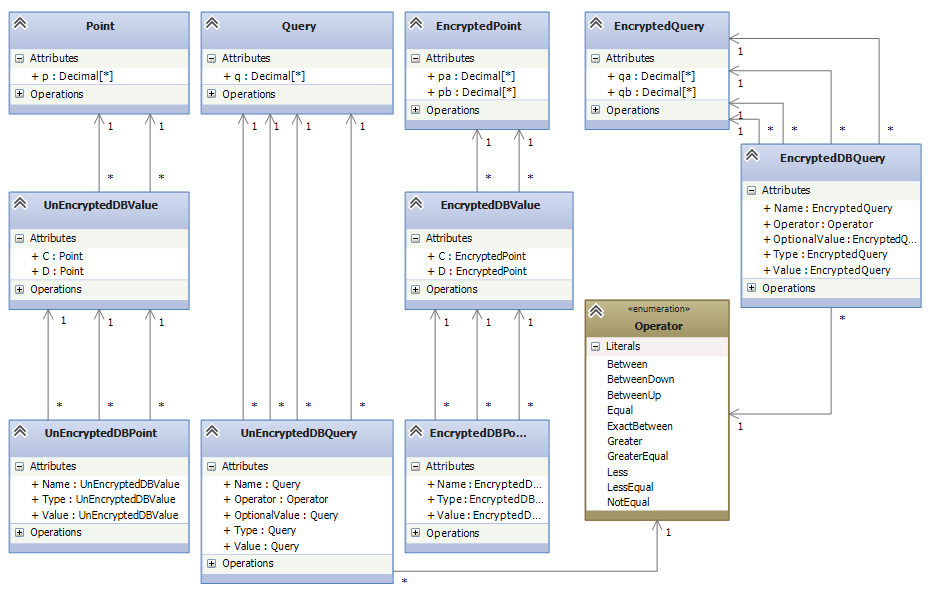
\includegraphics[angle = -90,scale = 3]{classdiagram}
\subsection{CRUD Operation}
Because ASPEDB should offer same operations as a regular DB we need to implement all CRUD\footnote{\url{https://en.wikipedia.org/wiki/Create,_read,_update_and_delete}} operations. In our case web server is considered trusted but curious so he will process our data corectly but will not alter or hide our data.
\subsubsection{Create}
\begin{figure}[h!]
 \centering
     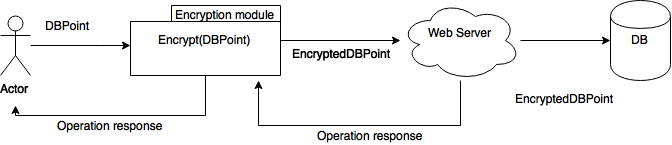
\includegraphics[width=0.9\textwidth]{InsertUseCase}
 \caption{Creation of a record use case.}
\end{figure}

When user wants to inset data in DB he creates a tuple $(Type,Name,Value)$ then each element in tuple is transformed in numeric value as is described in previous section. Now we support 3 data types :number,string,date. After conversion 3 points a generated so our tuple is now $(p_{Type},p_{Name},p_{Value})$ so now we can hide each element in a interval $[c,d]$ specific for each element so we generate $s_{Type},s_{Name},s_{Value}$ and we obtain $((c_{Type},d_{Type}),(c_{Name},d_{Name}),(c_{Value},d_{Value}))$. Now this tuple can be encrypted using EncryptionModule that uses fixed ASPE. Encrypted record \\ $((E(c_{Type}),E(d_{Type})),(E(c_{Name}),E(d_{Name})),(E(c_{Value}),E(d_{Value})))$ is inserted in database.
\subsubsection{Read}

\begin{figure}[h!]
 \centering
     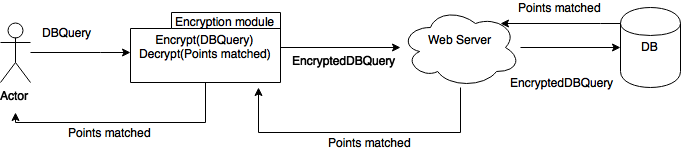
\includegraphics[width=0.9\textwidth]{searchusecase}
 \caption{Searching in db use case.}
\end{figure}
 When user wants to query database he choose data type of searching data ,name of data ,an operator to be applied on encrypted records, a value and optionally a second value if the operator chosen requires 2 values (for example $><,\geq<,>\leq,\geq\leq$). Each element in tuple except operator is transformed in number (same method as in creation of records) and transformed in query point. Each query point is encrypted by EncryptionModule using ASPE. so our encrypted query will be $(E(Type),E(Name),Operator,E(Value),E(OptionalValue))$ $OptionalValue$ is ecncrypted only in the case when it  exists otherwise it is set to $null$. This query is sent to web server to be processed. After query is processed client receives a list of encrypted points if there are points that are covered by query otherwise receives an empty list. If there are points user can recover them using EncryptionModule by decrypting them. so each element in list is now $((c_{Type},d_{Type}),(c_{Name},d_{Name}),(c_{Value},d_{Value}))$ to recover original point that are hiden in $[c,d]$ we will sum $c$ and $d$ so we will obtain $2p$ after that we recover encoded values from last position of point $p$ and decode it so we will obtain original tuple $(Type,Name,Value)$.
\subsubsection{Update}
\begin{figure}[h!]
 \centering
     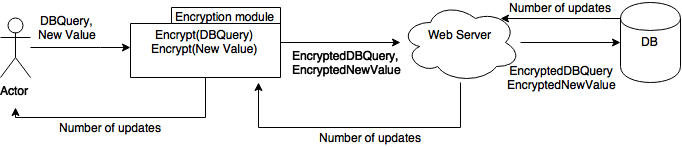
\includegraphics[width=0.9\textwidth]{updateusecase}
 \caption{Updating data in db use case.}
\end{figure}
Update operation will combine \textbf{Create} and \textbf{Read} so firs we will set a query to determine which points to update after that we create a new point that will  replace matched by the query. After we create query and new point data are sent to web server so server will replace matched records with new value and will count number of updated records and returns this value to user.
\subsubsection{Delete}
\begin{figure}[h!]
 \centering
     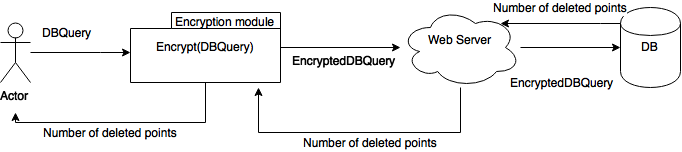
\includegraphics[width=0.9\textwidth]{deleteusecase}
 \caption{Deleting data in db use case.}
\end{figure}
Delete operation is similar to \textbf{Update} but instead of updating we will delete records matched by the query and count number of deleted records.
\section{Conclusion}
In conclusion we can say that KPA on ASPE can be fixed so ASPE can be used to secure outsourced databases that are managed by third parties .This fix is presented in current paper and a security proof also .  Unfortunately ASPE can't work well with strings and don't offers substring search. An advantage of ASPE is his scalability and queries over numeric values. 

ASPEDB presented in this work is a simple yet powerful application that allows users to execute CRUD operations on noSql databases.

Further work is to offer new functions over encrypted data and more complex queries. Also an interesting domain is to secure relational databases using ASPE.
\bigskip{}



\pagebreak{}


\begin{thebibliography}{4}
    \bibitem{Dormneco I.,Gavrilita C.}Dormenco I. Gavrilta C. Fixing KPA on ASPE(In progress)
	\bibitem{Wong}
	W. K. Wong, David W. Cheung, Ben Kao, Nikos Mamoulis, Secure kNN Computation on Encrypted Databases, 2009, Proceedings of the 2009 ACM SIGMOD International Conference on Management of data,
	Pages 139-152;
	\bibitem{Chunsheng} Gu Chunsheng, Gu Jixing, Known-plaintext attack on secure kNN computation on
	encrypted databases, SECURITY AND COMMUNICATION NETWORKS Security Comm. Networks 2014;7:2432–2441
	\bibitem{Choi} Sunoh Choi, Gabriel Ghinita, Elisa Bertino, A Privacy-Enhancing Content-Based Publish/Subscribe System Using Scalar Product Preserving, 2010, DEXA'10 Proceedings of the 21st international conference on Database and expert systems applications: Part I,
	Pages 368-384; 
	\bibitem{Joo} Jimmy Joo, NoSQL \& MongoDB
	\bibitem{Troelsen} Pro C\# 2010 and the .NET 4 Platform,exploring the universe using curly brackets:fith edition
\bibitem{Agrawal}Agrawal, R., Kiernan, J., Srikant, R., Xu, Y.: Order Preserving Encryption for Numeric
Data. In: ACM SIGMOD International Conference on Management of Data, pp. 563–574
(2004)
\bibitem{Boneh}Boneh, D., Waters, B.: Conjunctive, Subset, and Range Queries on Encrypted Data. In:
Theory of Cryptography Conference, pp. 535–554 (2007)
\end{thebibliography}
\end{document}
